\documentclass[12pt]{article}
\usepackage[utf8]{inputenc}
\usepackage[english,french]{babel}
\usepackage{geometry}
\usepackage{graphicx}
\usepackage{fancyhdr}
\usepackage{hyperref}

%% Links
\hypersetup{
    colorlinks,
    citecolor=black,
    filecolor=black,
    linkcolor=black,
    urlcolor=black
}

\geometry{hmargin=2cm, vmargin=2cm}

\def\blurb{TDDC32 - Analysis and Design Document 1.1}

\def\ligne#1{%
  \hbox to \hsize{%
    \vbox{\centering #1}}}%

\def\abstract{%
	This document give a complete description of the behavior of the Ray Tracing Engine. This project is the main part of the TDDC32 - Design and implementation of a software module in Java course.

This document include the system descriptions, the user interface. It also include all the functional and non functional requirements for this project. At the end of this document, you can see see the use cases descriptions.

The purpose of this document is not to discuss about implementation issues but focus on how the Ray Tracing Engine will be.


}

\makeatletter
\def\maketitle{%
	\null
	\vfill
	\vbox{\centering \Large \textbf{\blurb}}
	\vspace{15mm}
	\vbox{\centering \LARGE \textbf{\@title}}
	\vspace{15mm}
	\vbox{\centering \@author}
	\vspace{8mm}
	\vbox{\centering \@date}
	\vspace{15mm}
	\vbox{\centering \textbf{Abstract}}
	\vspace{5mm}
	\vbox{%
		\setlength{\fboxsep}{10pt}
		\centering \fbox{%
  		\begin{minipage}{0.9\textwidth}
  			\setlength{\parindent}{1cm}
  			\setlength{\parskip}{2ex plus .4ex minus .4ex}
	  		\abstract
  		\end{minipage}%
	  }
%
	}
	\vfill

}

\title{Ray Tracing Engine}
\author{Simon Vernhes \texttt{<simon@vernhes.eu>}}
\date{\today}

\begin{document}
  \selectlanguage{english}

  \pagestyle{fancyplain}
  \setlength{\parskip}{.6ex plus .4ex minus .4ex}
  \renewcommand{\headrulewidth}{0pt}
  \renewcommand{\footrulewidth}{0.6pt}
  \fancyhf{}
  \fancyhead{} 
  \lfoot{\blurb \\ \@title}
  \rfoot{Page \thepage}

  %% First page & table of content
  \maketitle \clearpage
  \tableofcontents \clearpage
 
  %% Content
  \section{Document conventions}

\begin{figure}[ht]
  \centering
  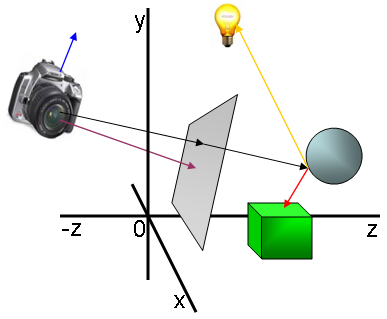
\includegraphics[height=7cm]{img/intro.png}
  \caption{Ray tracing}
\end{figure}

\begin{itemize}
  \item eye : camera
  \item viewport : plan where the eye is looking at
  \item shading effect : way to render/color a pixel (ray intersection with an object)
  \item scene : the scene the ray tracer have to render (described in the xml scene file)
\end{itemize}

  \clearpage
  \section{Class diagrams}

\begin{figure}[ht]
  \centering
  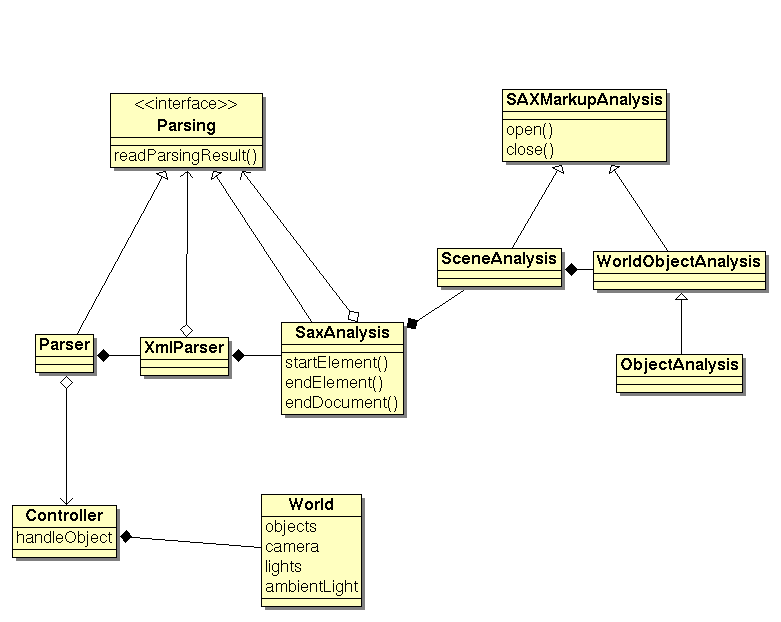
\includegraphics[height=15cm]{img/cd_parser.png}
  \caption{ray tracing parser}
\end{figure}

\begin{figure}[ht]
  \centering
  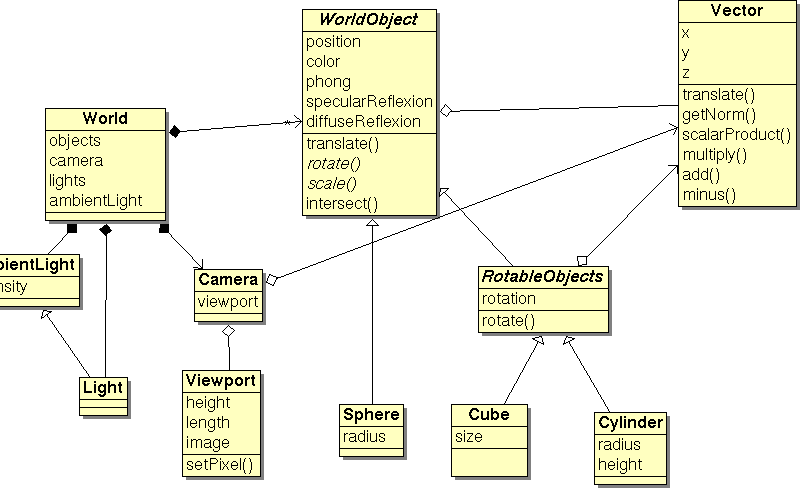
\includegraphics[height=10cm]{img/cd_wo.png}
  \caption{Ray tracing World Objects}
\end{figure}

\begin{figure}[ht]
  \centering
  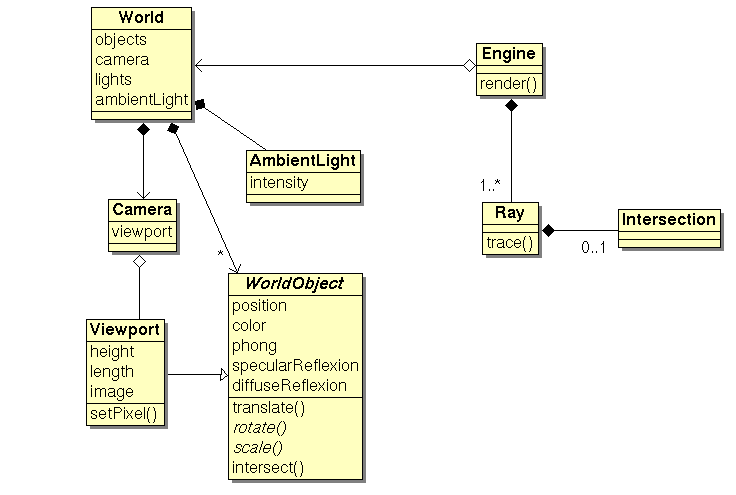
\includegraphics[height=10cm]{img/cd_engine.png}
  \caption{Ray tracing Engine}
\end{figure}


  \clearpage
  \section{Class descriptions}

  \subsection{Parser}

This set of classes will be created to use efficiency the SAX parser.

\begin{itemize}
  \item Controller : Receive all created object from parsing and add it to the World class. 
  \item Parsing : interface, describe a unique method "readParsingResult" to give back the newly created object from parsing to the parent class. Controller is the last called.
  \item Parser : prepare the xml parser.
  \item XMLParser : initialize SAX parser.
  \item SaxAnalysis : Sax Handler, analyse each markup sended by SAX and call the right SaxMarkupAnalysis class.
  \item SaxMarkypAnalysis : interface which describe a markup analyser
  \item *Analysis : one class for each markup, implementing SaxMarkupAnalysis. These classes create an object using given markup attributes.
\end{itemize}

  \subsection{World Objects}

\begin{itemize}
  \item Vector : 3D Vector (cartesian coordinates)
  \item WorldObject : abstract class use to describe a general object, this class is able to translate the center of the object. The intersect method return the point where a Ray inter
  \item RotableObject : abstract class, handle the possible rotation of object (derive from WorldObject).
  \item World : set of World Object with camera and ambient light and all other lights.
  \item AmbientLight : describe the ambient light, with RGB color.
  \item Light : derive from AmbientLight, these lights have a position.
  \item Sphere : describe a sphere by its center and its radius
  \item Cube : describe a cube by its position and its size
  \item Cylinder : describe a cylinder by its center, its radius and its height
  \item Camera : Position of the camera and it's direction. Create the Viewport for the future rendering

\end{itemize}

  \subsection{Engine}

The class Engine will use the World to render an image.

\begin{itemize}
  \item Intersection : describe an intersection between a Ray and a WorldObject with the distance from the origin of the ray and the position of the intersection, the normal to the surface and the WorldObject involved in this intersection.
  \item Ray : a ray which will be traced. Have an origin and a direction. The trace method will try to intersect with all the WorldObjects and return the closest intersection to the origin.
  \item Viewport : a 2D plan in front of the camera which represent the image. It contains a set of method to create the image. It can also create a dynamic visualisation of the current creation of the image.
  \item Renderer : The main algorithm of the Ray Tracer. It will cast a ray for each pixel of the Viewport and calculate the color of each pixel.
\end{itemize}


  \clearpage
  \section{Use case diagrams}
  \subsection{General view}
The user should call the ray tracer engine providing a scene xml file. The parser will create the world objects. And finally the engine will render the image using the world objects.

\begin{figure}[ht]
  \centering
  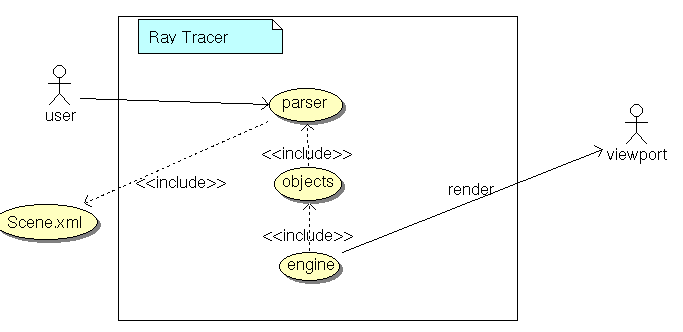
\includegraphics[height=9cm]{img/uc_raytracer.png}
  \caption{Use case general view}
  \label{img_uc_rt}
\end{figure}

  \clearpage
  \subsection{Objects}

The parser create all objects of the scene.

The creation of the camera also create the viewport.

\begin{figure}[ht]
  \centering
  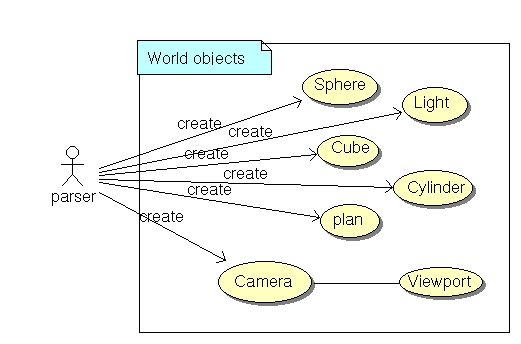
\includegraphics[height=9cm]{img/uc_objects.png}
  \caption{Use case objects creation}
  \label{img_uc_obj}
\end{figure}

  \clearpage
  \subsection{Engine}

Engine algorithm : for each pixel of the viewport, throw a ray and calculate the color where the ray intersect with an object.

\begin{figure}[ht]
  \centering
  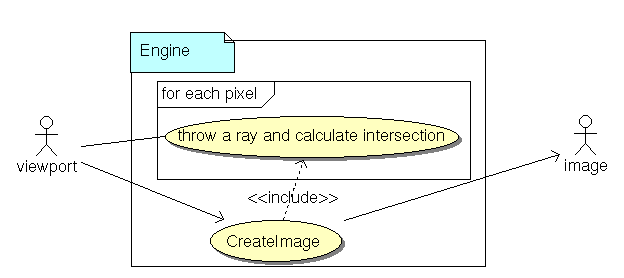
\includegraphics[height=7cm]{img/uc_render.png}
  \caption{Use case engine}
  \label{img_uc_engine}
\end{figure}


  \clearpage
  \section{Interaction diagrams}

\begin{figure}[ht]
  \centering
  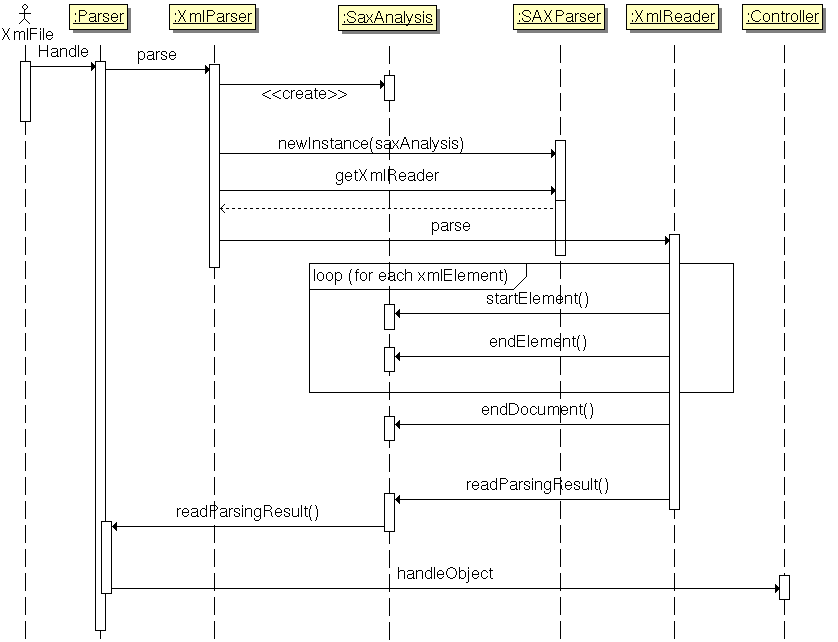
\includegraphics[height=15cm]{img/seq_parser.png}
  \caption{ray tracing parser}
\end{figure}




  \clearpage
  \section{State and Activity diagrams}

\begin{figure}[ht]
  \centering
  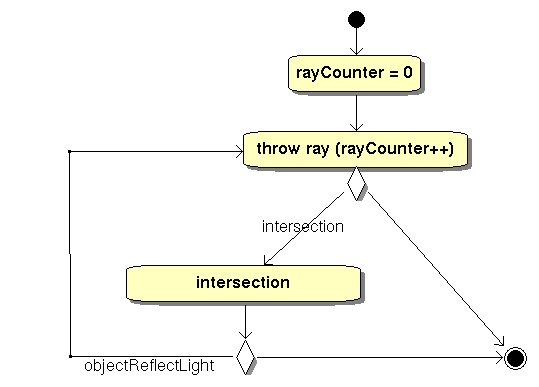
\includegraphics[height=10cm]{img/state_engine.png}
  \caption{ray tracing parser}
\end{figure}



  \clearpage
  \section{Test planning}

  \subsection{Unit Test}

Each WorldObject will be unit tested, mainly the intersect method (intersection of the object with a ray)

The ray tracing algorithm must be well tested before be really used. It cannot be really unit tested, mainly due to the fact that the result is an image, so it will be tested manually.

  \subsection{Integration test}


The parser must be test independently and be tested mostly manually.

Finally we can test some render with the complete program.


  \clearpage

\end{document}

